%%%%%%%%%%%%%%%%%%%%%%%%%%%%%%%%%%%%%%%%%%%%%%%%%%%%%%%%%%%%%%%
%% OXFORD THESIS TEMPLATE

% Use this template to produce a standard thesis that meets the Oxford University requirements for DPhil submission
%
% Originally by Keith A. Gillow (gillow@maths.ox.ac.uk), 1997
% Modified by Sam Evans (sam@samuelevansresearch.org), 2007
% Modified by John McManigle (john@oxfordechoes.com), 2015
% Modified by Ulrik Lyngs (ulrik.lyngs@cs.ox.ac.uk), 2018-, for use with R Markdown
%
% Ulrik Lyngs, 25 Nov 2018: Following John McManigle, broad permissions are granted to use, modify, and distribute this software
% as specified in the MIT License included in this distribution's LICENSE file.
%
% John commented this file extensively, so read through to see how to use the various options.  Remember that in LaTeX,
% any line starting with a % is NOT executed.  Several places below, you have a choice of which line to use
% out of multiple options (eg draft vs final, for PDF vs for binding, etc.)  When you pick one, add a % to the beginning of
% the lines you don't want.


%%%%% PAGE LAYOUT
% The most common choices should be below.  You can also do other things, like replacing "a4paper" with "letterpaper", etc.

% This one formats for two-sided binding (ie left and right pages have mirror margins; blank pages inserted where needed):
%\documentclass[a4paper,twoside]{templates/ociamthesis}
% This one formats for one-sided binding (ie left margin > right margin; no extra blank pages):
%\documentclass[a4paper]{ociamthesis}
% This one formats for PDF output (ie equal margins, no extra blank pages):
%\documentclass[a4paper,nobind]{templates/ociamthesis}

% As you can see from the uncommented line below, oxforddown template uses the a4paper size, 
% and passes in the binding option from the YAML header in index.Rmd:
\documentclass[a4paper, nobind]{templates/ociamthesis}


%%%%% ADDING LATEX PACKAGES
% add hyperref package with options from YAML %
\usepackage[pdfpagelabels]{hyperref}
% handle long urls
\usepackage{xurl}
% change the default coloring of links to something sensible
\usepackage{xcolor}

\definecolor{mylinkcolor}{RGB}{0,0,139}
\definecolor{myurlcolor}{RGB}{0,0,139}
\definecolor{mycitecolor}{RGB}{0,33,71}

\hypersetup{
  hidelinks,
  colorlinks,
  linktocpage=true,
  linkcolor=mylinkcolor,
  urlcolor=myurlcolor,
  citecolor=mycitecolor
}



% add float package to allow manual control of figure positioning %
\usepackage{float}

% enable strikethrough
\usepackage[normalem]{ulem}

% use soul package for correction highlighting
\usepackage{color, soulutf8}
\definecolor{correctioncolor}{HTML}{CCCCFF}
\sethlcolor{correctioncolor}
\newcommand{\ctext}[3][RGB]{%
  \begingroup
  \definecolor{hlcolor}{#1}{#2}\sethlcolor{hlcolor}%
  \hl{#3}%
  \endgroup
}
\soulregister\ref7
\soulregister\cite7
\soulregister\citet7
\soulregister\autocite7
\soulregister\textcite7
\soulregister\pageref7

%%%%% FIXING / ADDING THINGS THAT'S SPECIAL TO R MARKDOWN'S USE OF LATEX TEMPLATES
% pandoc puts lists in 'tightlist' command when no space between bullet points in Rmd file,
% so we add this command to the template
\providecommand{\tightlist}{%
  \setlength{\itemsep}{0pt}\setlength{\parskip}{0pt}}
 
% UL 1 Dec 2018, fix to include code in shaded environments

% User-included things with header_includes or in_header will appear here
% kableExtra packages will appear here if you use library(kableExtra)


%UL set section header spacing
\usepackage{titlesec}
% 
\titlespacing\subsubsection{0pt}{24pt plus 4pt minus 2pt}{0pt plus 2pt minus 2pt}


%UL set whitespace around verbatim environments
\usepackage{etoolbox}
\makeatletter
\preto{\@verbatim}{\topsep=0pt \partopsep=0pt }
\makeatother


%%%%%%% PAGE HEADERS AND FOOTERS %%%%%%%%%
\usepackage{fancyhdr}
\setlength{\headheight}{15pt}
\fancyhf{} % clear the header and footers
\pagestyle{fancy}
\renewcommand{\chaptermark}[1]{\markboth{\thechapter. #1}{\thechapter. #1}}
\renewcommand{\sectionmark}[1]{\markright{\thesection. #1}} 
\renewcommand{\headrulewidth}{0pt}

\fancyhead[LO]{\emph{\leftmark}} 
\fancyhead[RE]{\emph{\rightmark}} 

% UL page number position 
\fancyfoot[C]{\emph{\thepage}} %regular pages
\fancypagestyle{plain}{\fancyhf{}\fancyfoot[C]{\emph{\thepage}}} %chapter pages

% JEM fix header on cleared pages for openright
\def\cleardoublepage{\clearpage\if@twoside \ifodd\c@page\else
   \hbox{}
   \fancyfoot[C]{}
   \newpage
   \if@twocolumn\hbox{}\newpage
   \fi
   \fancyhead[LO]{\emph{\leftmark}} 
   \fancyhead[RE]{\emph{\rightmark}} 
   \fi\fi}


%%%%% SELECT YOUR DRAFT OPTIONS
% This adds a "DRAFT" footer to every normal page.  (The first page of each chapter is not a "normal" page.)

% IP feb 2021: option to include line numbers in PDF

% for line wrapping in code blocks
\usepackage{fvextra}
\DefineVerbatimEnvironment{Highlighting}{Verbatim}{breaklines,commandchars=\\\{\}}

% This highlights (in blue) corrections marked with (for words) \mccorrect{blah} or (for whole
% paragraphs) \begin{mccorrection} . . . \end{mccorrection}.  This can be useful for sending a PDF of
% your corrected thesis to your examiners for review.  Turn it off, and the blue disappears.
\correctionstrue


%%%%% BIBLIOGRAPHY SETUP
% Note that your bibliography will require some tweaking depending on your department, preferred format, etc.
% If you've not used LaTeX before, I recommend reading a little about biblatex/biber and getting started with it.
% If you're already a LaTeX pro and are used to natbib or something, modify as necessary.
% Either way, you'll have to choose and configure an appropriate bibliography format...

% this enables pandoc citations
\newlength{\cslhangindent}
\setlength{\cslhangindent}{1.5em}
\newlength{\csllabelwidth}
\setlength{\csllabelwidth}{3em}
\newlength{\cslentryspacingunit} % times entry-spacing
\setlength{\cslentryspacingunit}{\parskip}
\newenvironment{CSLReferences}[2] % #1 hanging-ident, #2 entry spacing
 {% don't indent paragraphs
  \setlength{\parindent}{0pt}
  % turn on hanging indent if param 1 is 1
  \ifodd #1
  \let\oldpar\par
  \def\par{\hangindent=\cslhangindent\oldpar}
  \fi
  % set entry spacing
  \setlength{\parskip}{1mm}
  \setlength{\baselineskip}{6mm}
 }%
 {}
\usepackage{calc}
\newcommand{\CSLBlock}[1]{#1\hfill\break}
\newcommand{\CSLLeftMargin}[1]{\parbox[t]{\csllabelwidth}{#1}}
\newcommand{\CSLRightInline}[1]{\parbox[t]{\linewidth - \csllabelwidth}{#1}\break}
\newcommand{\CSLIndent}[1]{\hspace{\cslhangindent}#1}




% Uncomment this if you want equation numbers per section (2.3.12), instead of per chapter (2.18):
%\numberwithin{equation}{subsection}


%%%%% THESIS / TITLE PAGE INFORMATION
% Everybody needs to complete the following:
\title{Fluid Responsiveness Prediction\\
During Surgery\\
\strut \\
\LARGE -- Physiological and Methodological\\
Limitations and Considerations\\}
\author{Johannes Enevoldsen}
\college{Health}

% Master's candidates who require the alternate title page (with candidate number and word count)
% must also un-comment and complete the following three lines:

% Uncomment the following line if your degree also includes exams (eg most masters):
%\renewcommand{\submittedtext}{Submitted in partial completion of the}
% Your full degree name.  (But remember that DPhils aren't "in" anything.  They're just DPhils.)
\degree{}
% Term and year of submission, or date if your board requires (eg most masters)
\degreedate{2022}


%%%%% YOUR OWN PERSONAL MACROS
% This is a good place to dump your own LaTeX macros as they come up.

% To make text superscripts shortcuts
	\renewcommand{\th}{\textsuperscript{th}} % ex: I won 4\th place
	\newcommand{\nd}{\textsuperscript{nd}}
	\renewcommand{\st}{\textsuperscript{st}}
	\newcommand{\rd}{\textsuperscript{rd}}

%%%%% THE ACTUAL DOCUMENT STARTS HERE
\begin{document}

%%%%% CHOOSE YOUR LINE SPACING HERE
% This is the official option.  Use it for your submission copy and library copy:
\setlength{\textbaselineskip}{22pt plus2pt}
% This is closer spacing (about 1.5-spaced) that you might prefer for your personal copies:
%\setlength{\textbaselineskip}{18pt plus2pt minus1pt}

% You can set the spacing here for the roman-numbered pages (acknowledgements, table of contents, etc.)
\setlength{\frontmatterbaselineskip}{17pt plus1pt minus1pt}

% UL: You can set the line and paragraph spacing here for the separate abstract page to be handed in to Examination schools
\setlength{\abstractseparatelineskip}{13pt plus1pt minus1pt}
\setlength{\abstractseparateparskip}{0pt plus 1pt}

% UL: You can set the general paragraph spacing here - I've set it to 2pt (was 0) so
% it's less claustrophobic
\setlength{\parskip}{2pt plus 1pt}

%
% Customise title page
%
\def\crest{{\includegraphics[width=5cm]{templates/AU\_SEGL/blue/ausegl\_blaa.pdf}}}
\renewcommand{\university}{Aarhus University}
\renewcommand{\submittedtext}{PhD dissertation}
\renewcommand{\thesistitlesize}{\fontsize{22pt}{28pt}\selectfont}
\renewcommand{\gapbeforecrest}{25mm}
\renewcommand{\gapaftercrest}{25mm}


% Leave this line alone; it gets things started for the real document.
\setlength{\baselineskip}{\textbaselineskip}


%%%%% CHOOSE YOUR SECTION NUMBERING DEPTH HERE
% You have two choices.  First, how far down are sections numbered?  (Below that, they're named but
% don't get numbers.)  Second, what level of section appears in the table of contents?  These don't have
% to match: you can have numbered sections that don't show up in the ToC, or unnumbered sections that
% do.  Throughout, 0 = chapter; 1 = section; 2 = subsection; 3 = subsubsection, 4 = paragraph...

% The level that gets a number:
\setcounter{secnumdepth}{2}
% The level that shows up in the ToC:
\setcounter{tocdepth}{1}


%%%%% ABSTRACT SEPARATE
% This is used to create the separate, one-page abstract that you are required to hand into the Exam
% Schools.  You can comment it out to generate a PDF for printing or whatnot.

% JEM: Pages are roman numbered from here, though page numbers are invisible until ToC.  This is in
% keeping with most typesetting conventions.
\begin{romanpages}

% Title page is created here
% Custom title page
\begin{titlepage}

\includegraphics[width=0.4\textwidth]{templates/AU\_LOGO/UK/BLUE/aulogo\_uk\_var2\_blue.pdf}
   
   \begin{center}
       \vspace*{1cm}

       {\huge \textbf{Fluid Responsiveness Prediction\\
During Surgery\\
\strut \\
\LARGE -- Physiological and Methodological\\
Limitations and Considerations\\}}

       %\vspace{0.5cm}
       %Thesis Subtitle
            
       \vspace{1.5cm}
       
       PhD dissertation

       {\large \textbf{Johannes Enevoldsen}}
       \vspace{0.8cm}
       
       \vfill
       
       \includegraphics[width=0.4\textwidth]{templates/AU\_SEGL/blue/ausegl\_blaa.pdf}
            
       \vspace{0.8cm}
     
            
       Health \\
       Aarhus University \\
       Department of Clinical Medicine \\
       2022
            
   \end{center}
\end{titlepage}

%%%%% DEDICATION
\begin{dedication}
  For my girls
\end{dedication}

%%%%% ACKNOWLEDGEMENTS


\begin{acknowledgements}
 	Thanks to my supervisor, Simon Tilma Vistisen, colleagues, family and friends, as well as Aarhus University and Holger \& Ruth Hesse's mindefond for founding this work.

  Also, thanks to all the kind strangers on the internet who selflessly helped me with various statistical and technical issues. Special thanks to John George Karippacheril, developer of \href{https://www.ncbi.nlm.nih.gov/pmc/articles/PMC3788264/}{VSCapture}, who helped me customize his software to work with department ventilators; essential for acquiring the data used in study 2 and study 3. Also, special thanks to Gavin L. Simpson, who after helping me with several issues posted on \textless stackoverflow.com\textgreater{} and Twitter, agreed to co-write the paper resulting from Study 2.

  \begin{flushright}
  Johannes Enevoldsen \\
  Aarhus University \\
  Fall, 2022
  \end{flushright}
\end{acknowledgements}



%%%%% ABSTRACT


\renewcommand{\abstracttitle}{Abstract}
\begin{abstract}
	Here is about one page of what this dissertation is about.
\end{abstract}




\renewcommand{\abstractsecondtitle}{Dansk Resumé}
\begin{abstractsecond}
	Her er et resume af afhandlingen.
\end{abstractsecond}


%%%%% MINI TABLES
% This lays the groundwork for per-chapter, mini tables of contents.  Comment the following line
% (and remove \minitoc from the chapter files) if you don't want this.  Un-comment either of the
% next two lines if you want a per-chapter list of figures or tables.
  \dominitoc % include a mini table of contents

% This aligns the bottom of the text of each page.  It generally makes things look better.
\flushbottom

% This is where the whole-document ToC appears:
\tableofcontents

\listoffigures
	\mtcaddchapter
  	% \mtcaddchapter is needed when adding a non-chapter (but chapter-like) entity to avoid confusing minitoc

% Uncomment to generate a list of tables:
%%%%% LIST OF ABBREVIATIONS
% This example includes a list of abbreviations.  Look at text/abbreviations.tex to see how that file is
% formatted.  The template can handle any kind of list though, so this might be a good place for a
% glossary, etc.
% First parameter can be changed eg to "Glossary" or something.
% Second parameter is the max length of bold terms.
\begin{mclistof}{List of Abbreviations}{3.2cm}

\item[AUROC]

Area under the receiver operating characteristic curve.

\item[CO]

Cardiac output.

\item[SV]

Stroke volume.

\item[SV]

Stroke volume.

\item[CI]

Compatibility interval, e.g 95\% CI {[}19.3; 25.2{]}. For Bayesian estimates, it is a \emph{credible interval}; for frequentist estimates, it is a \emph{confidence interval}. In both cases it represents the interval of parameter values compatible of the observed data.

\end{mclistof} 


% The Roman pages, like the Roman Empire, must come to its inevitable close.
\end{romanpages}

%%%%% CHAPTERS
% Add or remove any chapters you'd like here, by file name (excluding '.tex'):
\flushbottom

% all your chapters and appendices will appear here
\hypertarget{papers}{%
\chapter*{Papers}\label{papers}}
\addcontentsline{toc}{chapter}{Papers}

\adjustmtc
\markboth{Papers}{}

This PhD dissertation is based upon the following three papers:

\begin{itemize}
\tightlist
\item
  \textbf{Paper 1} Existing fluid responsiveness studies using the mini-fluid challenge may be misleading: Methodological considerations and simulations.
  \emph{\href{https://doi.org/10.1111/aas.13965}{Published in Acta Anaesthesiologica Scandinavica, 2021. DOI: 10.1111/aas.13965}.}
\item
  \textbf{Paper 2} Using generalized additive models to decompose time series and waveforms, and dissect heart--lung interaction physiology.
  \emph{\href{http://https://doi.org/10.1007/s10877-022-00873-7}{Published in Journal of Clinical Monitoring and Computing, 2022. DOI: 10.1007/s10877-022-00873-7}.}
\item
  \textbf{Paper 3}
\end{itemize}

\begin{savequote}
Medicine is a science of uncertainty and an art of probability.
\qauthor{--- \textbf{Sir William Osler} (1849--1919).}\end{savequote}



\hypertarget{introduction}{%
\chapter{Introduction}\label{introduction}}

Fluid therapy is a ubiquitous medical intervention; both in the perioperative setting and for hospitalised patients in general. The aim of fluid therapy is to restore the patient's circulating blood volume to the \emph{optimum}, normal, level. Hence, the terms ``fluid \emph{resuscitation}'' and ``fluid \emph{replacement} therapy'' are commonly used.

Intraoperative fluid management is mainly relevant in acute or long-duration surgery.
In acute surgery, the preoperative fluid status is generally unknown, and it is often reasonable to assume that the patient arrives at the operating room dehydrated.
In long-duration surgery, continuous loss of fluid through bleeding, perspiration and urination necessitates fluid replacement through the operation. Since these patients are anaesthetised, intravenous (IV) is the administration route of choice.

Like every treatment, IV fluid should only be given to patients who will benefit from the fluid.
This is the setup for a prediction problem: can we, ahead of time, predict whether a patient will benefit from an intravenous fluid administration?
The first task is to define what we mean with \emph{benefit}, and how we can measure it. This is not trivial, and it will be discussed further in section \ref{why-fluid}.
Luckily, a necessary (but not sufficient) condition for benefitting from a fluid administration is that the fluid causes an increase in cardiac output (CO).
This can be measured, and allows us to formulate a simpler prediction problem:

Can we predict whether a patient's CO will increase from a fluid administration?

There is an entire subfield of anaesthesia and intensive care research dealing with this problem.
This PhD dissertation describes a small, but hopefully meaningful addition to the field.

In this dissertation, I present the available tools for fluid responsiveness prediction, with focus on the intraoperative setting. The dissertation covers 3 papers that tackle specific limitations to the most common tools.

The terms \emph{fluid challenge} and \emph{bolus} are used interchangeably. \emph{Stroke volume} (SV) and \emph{cardiac output} (CO) are often interchangeable and the term that best fits the context is used. Ventilation and respiration is also used interchangeably and refer to the act of breathing (either mechanically or spontaneously).

\begin{savequote}
The most wonderful and satisfactory effect is the immediate consequence
of the injection {[}of fluid{]}. To produce the effect referred to, a
large quantity must be injected---from five to ten pounds in an
adult---and repeated at longer or shorter intervals, as the state of the
pulse, and other symptoms, may indicate.
\qauthor{--- \textbf{Robert Lewins, M.D.}, 1832 (Injection of Saline Solutions Into the Veins).}\end{savequote}



\hypertarget{background}{%
\chapter{Background}\label{background}}

\hypertarget{history}{%
\section{History}\label{history}}

Intravenous fluid therapy first became popular in the cholera epidemic around 1830, when Thomas Latta ``threw'' several litres of saline into the veins of severely dehydrated cholera patients, and Robert Lewins reported enthusiastically on the ``most wonderful and satisfactory effect'' {[}\protect\hyperlink{ref-lattaMALIGNANTCHOLERADOCUMENTS1832}{7},\protect\hyperlink{ref-lewinsInjectionSalineSolutions1832}{8}{]}. After the end of the epidemic, the treatment was mostly abandoned. Possibly because the early clinical reports from the epidemic mainly presented temporary effects and mostly in morbidly dehydrated patients, and also because the concerns raised by sceptics were probably highly relevant: the fluid was both unsterile and hypotonic {[}\protect\hyperlink{ref-cosnettOriginsIntravenousFluid1989}{3}{]}.

Interest in fluid resuscitation reemerged nearly 50 years later, in 1879, when Kronecker and Sander demonstrated the importance of volume (as opposed to red blood cells) in the treatment of haemorrhage: They bleed down two dogs until bleeding stopped from lack of cardiac activity (approx. 50 \% of the blood volume). Then, they reported how resuscitation with an equivalent volume of a saline solution would recover the animals' cardiac activity {[}\protect\hyperlink{ref-foexHowCholeraEpidemic2003}{4},\protect\hyperlink{ref-petroianuSalineInfusionClonus2021}{11}{]}. This was followed by a number of reports of successful IV fluid resuscitations in humans {[}\protect\hyperlink{ref-foexHowCholeraEpidemic2003}{4}{]}.

Since the end of the nineteenth century, IV fluid administration has been a staple in the treatment of the acutely ill and during surgery. With better equipment and hygiene, the safety of IV fluid administration has increased, and the indication for treatment has widened accordingly---today, IV fluid is even available as a drop-in or home-delivery hangover remedy {[}\protect\hyperlink{ref-kadetHouseCallsHangovers2015}{6}{]}. Naturally, debates about the appropriate use of IV fluids continue.

\hypertarget{why-fluid}{%
\section{Why give IV fluids?}\label{why-fluid}}

Fluid should only be administered when the patient is likely to benefit from it {[}\protect\hyperlink{ref-millerPerioperativeFluidTherapy2019}{9}{]}. As a treatment for hypovolemia, the goal is that the infused fluid will increase the circulating volume and thereby the mean systemic pressure. This gives an increase in cardiac preload and, through the Frank-Starling mechanism (see section ref:frank-starling), an increase in CO. This should increase microcirculation and, in turn, the oxygen available to organs, increasing (or retaining) organ function (see Figure \ref{fig:background-monnet2018-aic-fluid2organ}) {[}\protect\hyperlink{ref-monnetMyPatientHas2018}{10}{]}. As discussed in section ref:fluid-bolus-physiology, this goal is not always achieved.

\begin{figure}

{\centering 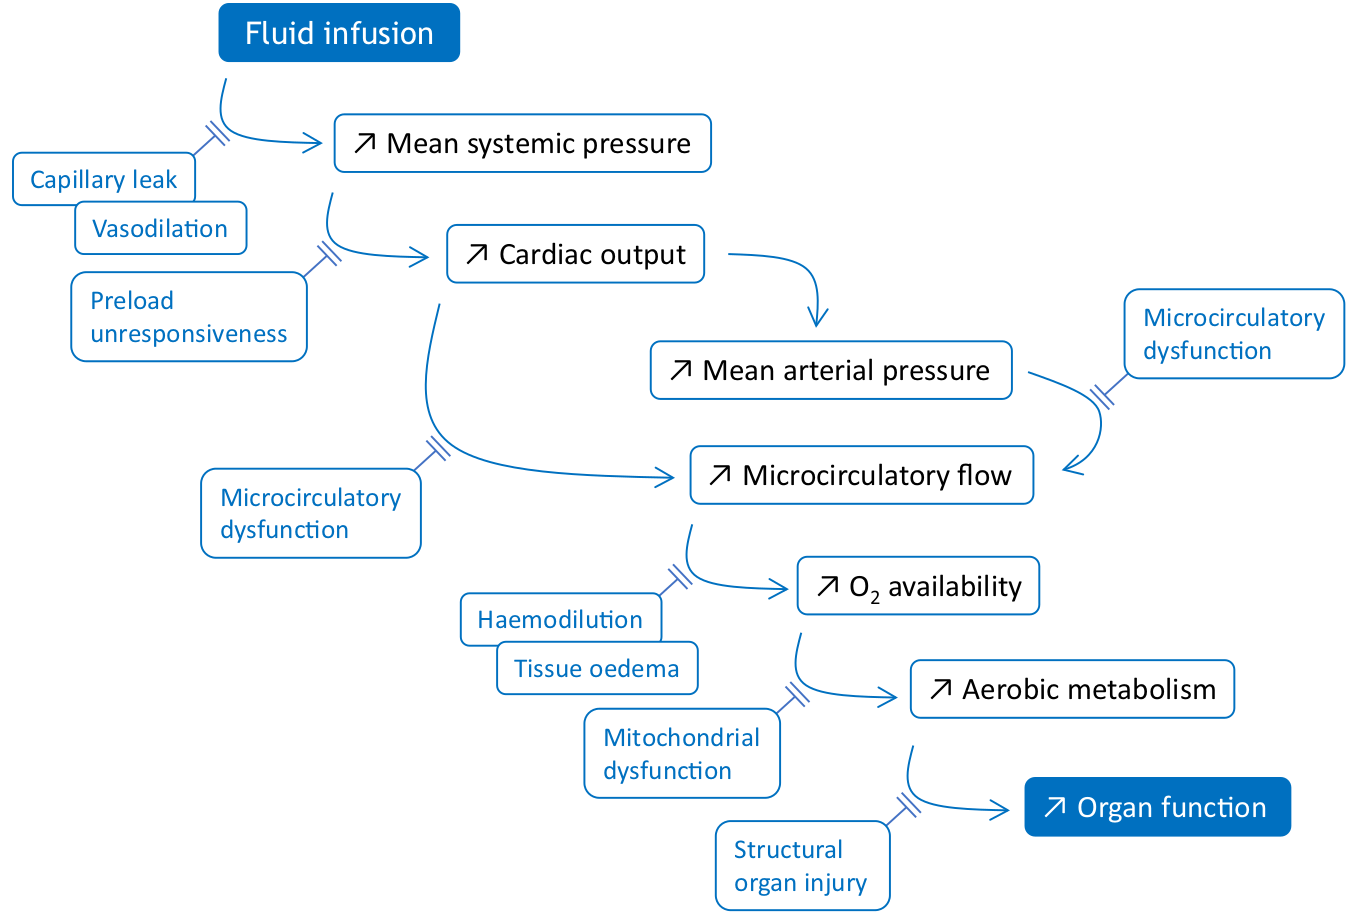
\includegraphics[width=14cm]{figures/background-monnet2018-aic-fluid2organ} 

}

\caption[Steps from fluid administration to benefit]{Illustration of the physiological steps from fluid administration to benefit. Reprinted from Monnet et al, 2018 {[}\protect\hyperlink{ref-monnetMyPatientHas2018}{10}{]} (\href{https://creativecommons.org/licenses/by/4.0/}{CC BY}).}\label{fig:background-monnet2018-aic-fluid2organ}
\end{figure}



Another common aim with IV fluid therapy is to resuscitate dehydration, characterised by hypertonicity (excess salt) due to loss of water---e.g., due to gastroenteritis or diabetic polyuria. While hypovolemia can be corrected rapidly with IV infusion of an isotonic fluid, hypertonicity should be corrected slowly through oral intake of water or with IV hypotonic fluid {[}\protect\hyperlink{ref-bhaveVolumeDepletionDehydration2011}{1}{]}. This dissertation focuses on fluid as a treatment of hypovolemia, and dehydration/hypertonicity will not be discussed further.

During surgery, there is a continuous loss of circulation fluid through urination, bleeding, perspiration and \emph{redistribution}. If this fluid is not replaced, the patient will gradually become hypovolemic and, eventually, organ failure will occur. Since blood loss and urination is accurately recorded throughout the surgery, the unknown volume of fluid to replace is from perspiration and redistribution {[}\protect\hyperlink{ref-jacobThirdSpaceFact2009}{5}{]}. An additional unknown is the patient's fluid status on arrival to the operating room. Preoperative hypovolemia due to extended fasting before operations used to be a relevant concern, and was treated with significant volumes of fluid during or before induction of anaesthesia {[}\protect\hyperlink{ref-coeCrystalloidPreloadingUseful1990}{2},\protect\hyperlink{ref-jacobThirdSpaceFact2009}{5}{]}. With today's more liberal guidelines for pre-surgery fluid intake, allowing clear fluids until two hours before surgery, the preoperative deficit is probably lower {[}\protect\hyperlink{ref-jacobThirdSpaceFact2009}{5},\protect\hyperlink{ref-millerPerioperativeFluidTherapy2019}{9},\protect\hyperlink{ref-smithPerioperativeFastingAdults2011}{12}{]}.

With the risk of organ failure from hypovolemia, why not simply give the patient some extra fluid to ensure that there is enough?
\#\# Concerns about liberal use of IV fluids

The statement that IV fluid administration should be treated as any other prescription medication has become a trope in fluid resuscitation literature {[}cite miller 2019; Myburgh 2013; Hoste 2014; Malbrain 2020{]}. For good reasons. In addition to the intended effect summarised in the section above, fluid administration can cause side effects. The principal concerns with excessive fluid administrations can be divided into hypervolemia and non-volume-related effects. The non-volume-related effects depend on the type of fluid. Notable examples include hyperchloremic acidosis from normal saline and kidney injury associated with excessive? HES infusion {[}cite Myburg 2013; perner 2012{]}. Hypervolemia is a more general issue with excessive fluid administration, causing oedemas of tissue and lungs. The pathophysiology of hypervolemia involves both cardiovascular mechanics and microcirculation, so this will be a good place for an introduction to the physiology related to fluid administrations.

\hypertarget{fluid-bolus-physiology}{%
\section{The physiology and pathophysiology of a fluid bolus}\label{fluid-bolus-physiology}}

A fluid bolus should increase stroke volume (SV) and, hence, CO. This requires that the fluid remains in circulation to increase cardiac preload, and that this increase in cardiac preload causes an increase in SV. We will start with the latter condition: the Frank-Starling mechanism.
\#\#\# The Frank-Starling mechanism \{\#frank-starling\}

The relation between cardiac preload and SV is often termed the ``Frank-Starling mechanism'' or the ``Frank-Starling law of the heart'', after Otto Frank and Ernest Starling, who are commonly attributed the discovery of the relationship {[}cite frank1895; patterson1914{]}. It has been noted, though, that the phenomenon had been observed several decades earlier {[}cite zimmer2002{]}. The Frank-Starling mechanism describes that increasing the length of a cardiomyocyte will increase the force generated when the muscle is activated; or, as a consequence, that increased filling of a ventricle will increase stroke volume. The relation occurs only until a certain length/volume, where the curve flattens and the effect eventually reverses. This was clearly demonstrated in experiments by Otto Frank, where he measured the pressure generated through isovolumetric contractions of frog hearts (see figure ref:background-frank1895).

(Figure: background-frank1895): Otto Frank's tracings of intraventricular pressure during isovolumetric contractions. In each panel, ventricular volume increases with the number on the tracing. Right panel, tracing 4 demonstrates the decrease in maximum pressure with overdistension. Reproduction of figures from Frank 1895, {[}cite frank1895{]} public domain.

A clinical consequence of the Frank-Starling mechanism is that a patient's SV can only increase from a fluid bolus, if the heart is currently functioning on the rising section of the Frank-Starling curve (see figure ref:background-starling-curve). A heart's Frank-Starling curve is, however, not constant, but can be raised with higher sympathetic tone or sympathomimetic drugs (positive inotropes).

(Figure: background-starling-curve): Illustration of the Frank-Starling mechanism---the relation between the end-diastolic volume and the stroke volume. If end-diastolic volume is increased in a heart operating on the steep part of the curve (e.g.~by a fluid bolus) stroke volume will increase. If the heart is already operating on the flat part of the curve, no increase in stroke volume can be expected.

A few concepts are used interchangeably for both the cause and the effect in the Frank-Starling relationship. Starling et al.~note that the physiological relationship must be between the length of a piece of cardiac muscle and the tension it exerts when it contracts, but, since they are not able to measure these in an intact heart, assume that ventricular volume is linearly related to muscle length, and that ventricular pressure is linearly related to muscle tension. They appropriately note that this assumption will become increasingly incorrect with distension and a more globular shape of the ventrice {[}cite patterson1914{]}. Other terms used as proxies for end-diastolic muscle length are preload and end-diastolic pressure. Preload should be synonymous with end-diastolic volume or muscle length, but the term is often not well defined. End-diastolic pressure is of course related to muscle length, but it also depends on static mechanical factors (e.g.~fibrosis), external pressure and the shape and size of the heart. Proxies for the systolic muscle tension include afterload, systolic ventricular pressure, stroke volume and mechanical work.
\#\#\# Venous return and mean systemic filling pressure
In steady state, blood circulates continuously from the heart to the arteries, through tissues, to the veins and back to the heart. The circulating volume is constant and CO is equal to the venous return to the heart. We can consider a simple model of this system, where blood is pumped from a small elastic compartment into a larger elastic compartment and returned again to the smaller elastic compartment through a tube (see figure \{ref:background-venous-return-simple). The pump is the heart, the large compartment represents the capacitance of venules and veins---completely neglecting the capacitance of the arteries---and the smaller compartment represents the right atrium and large veins immediately upstream from the heart. Arteries are neglected in this model because of their low compliance relative to the venous system (for an illustration of how the arterial system would fit in this model, see figure fig:background-venous-return-art) {[}cite magder 2016 volume{]}. The pressure in the large compartment is the venous pressure (P\textsubscript{V}), the pressure in the smaller compartment is the right atrial pressure (P\textsubscript{RA}) and the resistance in the tube is the resistance to venous return (R\textsubscript{V}). If the pump is stopped, both compartments will reach an equilibrium pressure: the mean systemic filling pressure (P\textsubscript{MSF}).

(Figure: background-venous-return-simple): A simple model illustrating the concepts of venous return (Q\textsubscript{V}) and mean systemic filling pressure (P\textsubscript{MSF}). The pressure is defined by the height of the fluid surface and the compliance is proportional to the width of the compartment. CO, cardiac output. P\textsubscript{V}, pressure of the compartment representing venules and veins. R\textsubscript{V}, resistance to venous return. P\textsubscript{RA}, pressure of the compartment representing the right atrium.

(Figure: background-venous-return-art): An illustration of how the arterial system could be represented in the simple model illustrated in figure fig:background-venous-return-simple. MAP, mean arterial pressure.

From this simple model, we can appreciate some factors that determine CO. First, the heart's ability to pump is the absolute limitation to cardiac output. However, the heart also cannot pump more than what is returned from the veins. This venous return is determined by the resistance to venous return and the pressure difference between the venous compartment and the right atrial compartment:

\[
CO = Q_V = \frac{P_V - P_{RA}}{R_V}.
\]

Thus, increasing venous pressure or lowering resistance to venous return \emph{allows} a higher CO. If venous compliance is constant, a fluid bolus can increase venous pressure. Alternatively, we can use an \(\alpha\)-adrenergic agonist such as noradrenaline to decrease venous compliance and thereby increase pressure without adding fluid (venoconstriction will also increase resistance to venous return, but the effect on compliance seems to dominate) {[}cite persichini2022{]}. Models of venous return often divide compartments into stressed volume and unstressed volume. The unstressed volume is the volume of fluid that will not create any pressure in the compartment---essentially the volume that will remain if the circulation is lacerated. Unstressed volume is effectively inert, and only the stressed volume has any influence on venous return. Unstressed volume can, however, become stressed through vasoconstriction. While the concept of unstressed volume makes sense anatomically (a vessel can be filled to a certain volume without exerting an elastic recoil), it will often be difficult to differentiate between the effects of \emph{unstressed volume becoming stressed} and ``a decrease in compliance of already stressed volume* (both increase P\textsubscript{MSF}).

As described in the section above, the Frank-Starling curve describes the relationship between ventricular filling and CO (via SV). Ventricular filling is positively related to the right atrial pressure, while the right atrial pressure is inversely related to CO, since a high CO will tend to empty the right atrial compartment. The right atrial pressure and CO where venous return and cardiac output are in equilibrium can be found as the intersection between the venous return curve (the relationship between venous return and right atrial pressure) and a variant of the Frank-Starling curve with CO rather than SV on the y-axis (see figure fig:guyton). This graphical solution was first proposed by Arthur Guyton {[}cite Guyton1957{]}.

(Figure: background-guyton): A) The relationship between venous return (Q\textsubscript{V}), right atrial pressure (P\textsubscript{RA}) and cardiac output (CO). If CO (and hence Q\textsubscript{V}) drops to zero, P\textsubscript{RA} will equal the mean systemic filling pressure (P\textsubscript{MSF}). The circulation is at steady state at the intersection of the venous return function and the cardiac function (when Q\textsubscript{V} = CO). This illustration corresponds to spontaneous breathing, where the intrathoracic pressure is negative. Therefore, the cardiac function starts at a negative pressure where the ventricular transmural pressure (P\textsubscript{tm,RV}) is zero. B) Change in inotropy or heart rate. C) Change in resistance to venous return (R\textsubscript{V}). D) Change in P\textsubscript{MSF}; either via change in stressed volume or compliance of capacitance vessels.

The simple model depicted in figure fig:venous-return-simple and Guyton's graphical solution the steady state CO, provides a basis for understanding clinical interventions that impact CO. One category of interventions target the heart directly by increasing inotropy or chronotropy (increase in cardiac function). A common drug with this effect is dobutamine, which has both positive inotrope and chronotrope effects. In isolation, positive inotropy or chronotropy will increase CO and lower P\textsubscript{RA}, as depicted in figure fig:guyton B. From this figure, we can also identify the theoretical maximum CO obtainable from inotropy or chronotropy: when the heart essentially pumps the right atrium ``dry'' faster than the venous return can refill it. Since veins are flaccid, they cannot have a transmural pressure below zero. Lowering P\textsubscript{RA} below zero (only possible because the intrathoracic pressure is below zero) will not further increase venous return as extrathoracic veins will collapse in proportion to the lower P\textsubscript{RA} (depicted as the left steady state point in figure fig:guyton B). This is known as the ``waterfall effect'', since it is analogous to how changing the lower water level in a waterfall will not affect the flow over the waterfall (cite:Permutt1963).

A second target for optimising CO, is resistance to venous return (R\textsubscript{V}). This resistance can be greatly increased with liver cirrhosis, and alleviation by transjugular intrahepatic portosystemic shunt (TIPS) increases CO (cite: wong1995). Late stages of pregnancy can also increase R\textsubscript{V} via compression of the inferior vena cava when the mother is in supine position. Increase in R\textsubscript{V} does not impact P\textsubscript{MSF} but reduces P\textsubscript{RA} and thereby CO (see figure fig:guyton C).

The last point of intervention is P\textsubscript{MSF}. A fluid bolus will increase P\textsubscript{MSF} by increasing stressed volume while maintaining compliance of capacitance veins. Venoconstriction (e.g.~with noradrenaline) decreases compliance of capacitance veins, and may additionally mobilise previously unstressed volume; both effects increase P\textsubscript{MSF}. An increase of P\textsubscript{MSF} increases P\textsubscript{RA} and thereby CO on the condition that the heart is operating on the ascending part of the Frank-Starling curve (see figure fig:guyton C).
\#\#\# Fluid distribution and oedema formation

A principal adverse effect of fluid administration is oedema: a pathological build-up of fluids in the intercellular tissue or within alveoli. Additional fluid in the interstitium increases the diffusion distance between the capillary blood and the cells, decreasing the rate of oxygen delivery to the mitochondria {[}cite dunn2016{]}. Pulmonary oedema has a similar detrimental effect on gas exchange in the alveoli.

\hypertarget{the-classic-understanding-of-oedema-formation}{%
\subsubsection{The classic understanding of oedema formation}\label{the-classic-understanding-of-oedema-formation}}

The mechanism for oedema formation is classically described with Ernest Starling's understanding of capillary physiology: The interstitial fluid is in an equilibrium between the colloid-osmotic (oncotic) pressure from the macromolecules in blood (pull) and the hydrostatic pressure across the capillary membrane (push). An increase in stressed volume increases transcapillary pressure, driving fluid into the interstitium until a new equilibrium is reached {[}cite boronMicrocirculation2016{]}. Adding to this, crystalloid fluids (e.g.~normal saline or acetated Ringer's solution) dilute plasma, which lowers the oncotic pressure and further promotes the formation of oedema.

\hypertarget{a-revised-mechanism-of-oedema-formation-the-endothelial-glycocalyx}{%
\subsubsection{A revised mechanism of oedema formation: the endothelial glycocalyx}\label{a-revised-mechanism-of-oedema-formation-the-endothelial-glycocalyx}}

In recent years, increasing focus has been on the endothelial glycocalyx layer's role in fluid resuscitation and oedema formation. The glycocalyx is a gel of macromolecules (mainly glycoproteins, hyaluronans and proteoglycans) lining the vascular endothelium (cite:weinbaum2007). One function of this layer is to form a semipermeable membrane that, in addition to retaining plasma proteins, also retains water to a variable degree. In this model, the flow of water from vaculatere to tissue is determined less by oncotic pressure difference and more by the current state of the glycocalyx layer (cite:milfordRecusitationfluid2019). The permeability of the glycocalyx layer may be impacted by volume loading. A proposed mechanism for this regulation is that volume loading increases right atrial pressure, causing release of atrial natriuretic peptide (ANP). ANP increases water filtration and may, directly or indirectly, damage the glycocalyx (chappallHypervolemia2014). This mechanism has, however, later been questioned (cite:damenAtrial2021). Another important cause of glycocalyx degradation is inflammation---especially related to sepsis (cite:ibaDerangement2019).

\hypertarget{how-long-does-fluid-remain-in-circulation}{%
\subsubsection{How long does fluid remain in circulation?}\label{how-long-does-fluid-remain-in-circulation}}

Fluids must remain in circulation to benefit the patient's hemodynamic status. Both patient and fluid specific factors impact how long we can expect a fluid bolus to exert its intended effect. The intravascular half-life of a crystalloid infusion is around 20 to 40 minutes in conscious volunteers, while the half-life is more than doubled in surgery with general anaesthesia. Colloids are reported to expand plasma volume with a half-life of two to three hours for both healthy subjects and during surgery (the half-life of the macromolecules themselves in synthetic starches (HES) are much longer than the effect on volume expansion). Generally, a hypovolemic state is associated with a more persistent effect of a volume expansion (cite: hahnHalflife2016).

\hypertarget{how-much-fluid-should-we-give-and-when}{%
\section{How much fluid should we give and when?}\label{how-much-fluid-should-we-give-and-when}}

There are two overall strategies for fluid management: to replace fluids according to an estimated loss or deficit, or to give fluids until a specific hemodynamic target is reached.

The fluid replacement strategy is commonly investigated by comparing a \emph{restrictive} strategy against a \emph{liberal} strategy. The terms \emph{restrivive} and \emph{liberal} are, of course, relative, and through years with superior results from \emph{restrictive} fluid regiments, both terms have referred to successively lower volumes. This trend seems to have been concluded with the RELIEF trial (cite: millerPerioperative2019).

In the RELIEF trial, 3000 patients undergoing abdominal surgery were randomised to either a \emph{liberal} fluid regiment, expected to give a positive fluid balance, or to a \emph{restrictive} fluid regiment, expected to give a neutral fluid balance. The \emph{liberal} group received a median of 6.1 litres of fluid, while the \emph{restrictive} group received a median of 3.7 litres. There was no difference in disability-free survival between the groups, but the \emph{restrictive} group had a higher rate of acute kidney injury. The \emph{liberal} group had a calculated fluid balance of +3.1 litres and gained 1.6 kg weight; the \emph{restrictive} group had a +1.4 litre fluid balance and gaind 0.3 kg (weight gain was only measured in one third of the patients). (mylesRestrictive2018) Overall, this suggests that a positive fluid balance of 1-2 litres is preferable in major abdominal surgery (cite brandstrupFinding2018).

The alternative---or complementary---strategy is goal directed hemodynamic therapy (GDT). Here, patients are treated with fluid, and often vasopressors, to reach a specific hemodynamic target. The aim with GDT is to individualise treatment to ensure that hypovolemic patients get enough fluid, while avoiding fluid overload. A common GDT target is CO optimisation: fluid is given in boluses until CO stops increasing. This is interpreted ast the patient's heart having reached the plateau top of the Frank-Starling curve, and that further fluid administration will be futile. An example of GDT was investigated in the OPTIMISE trial (cite: pearseEffect2014).

The OPTIMISE trial randomised 724 high-risk, abdominal surgery patients to either CO-guided GDT or \emph{usual care}. The GDT intervention consisted of a fluid administration algorithm where first, a patient's target SV was determined by administering colloid fluid in 250 ml boluses until a new bolus no longer caused a sustained increase in SV above 10\%. Afterwards, fluids were administered to maintain this target SV. Additionally, dopexamine (inotrope) was infused at a low rate (0.5 µg kg\textsuperscript{-1} min\textsuperscript{-1}). The study results were inconclusive: they were suggestive of a protective effect of the GTD protocol on adverse events and mortality, though the results were also compatible with there being no difference between groups.

Generally, the effect of GDT is difficult to assess. Both because protocols are numerous and heterogenous and because \emph{usual care} continues to assimilate the GDT protocols under investigation (cite: millerPerioperative2019). A recent systematic review of 76 randomised GDT trials had a conclusion similar to the OPTIMISE trial: GDT might work (cite: jessenGoaldirected2022).

There are some disadvantages to the SV-optimising approach to fluid therapy. First, it requires continuous monitoring of SV or CO. Recent technological advances have broadened the availability of continuous CO monitoring, though the accuracy of these technologies are debated (see section (ref:methods-co)). Second, it can be (??has been) argued that if fluid is given until it no longer increases SV, then the last fluid bolus was unnecessary and should not have been given. This could be avoided, if the response to a fluid bolus could be predicted.

\startappendices

\hypertarget{paper-1}{%
\chapter{Paper 1}\label{paper-1}}

\newpage \begin{center} \makebox[\linewidth][c]{\includegraphics[width=1.2\linewidth]{papers/paper1//page-1.pdf}} \end{center} \newpage \begin{center} \makebox[\linewidth][c]{\includegraphics[width=1.2\linewidth]{papers/paper1//page-2.pdf}} \end{center} \newpage \begin{center} \makebox[\linewidth][c]{\includegraphics[width=1.2\linewidth]{papers/paper1//page-3.pdf}} \end{center} \newpage \begin{center} \makebox[\linewidth][c]{\includegraphics[width=1.2\linewidth]{papers/paper1//page-4.pdf}} \end{center} \newpage \begin{center} \makebox[\linewidth][c]{\includegraphics[width=1.2\linewidth]{papers/paper1//page-5.pdf}} \end{center} \newpage \begin{center} \makebox[\linewidth][c]{\includegraphics[width=1.2\linewidth]{papers/paper1//page-6.pdf}} \end{center} \newpage \begin{center} \makebox[\linewidth][c]{\includegraphics[width=1.2\linewidth]{papers/paper1//page-7.pdf}} \end{center} \newpage \begin{center} \makebox[\linewidth][c]{\includegraphics[width=1.2\linewidth]{papers/paper1//page-8.pdf}} \end{center}

\hypertarget{paper-2}{%
\chapter{Paper 2}\label{paper-2}}

\newpage \begin{center} \makebox[\linewidth][c]{\includegraphics[width=1.2\linewidth]{papers/paper2//page-1.pdf}} \end{center} \newpage \begin{center} \makebox[\linewidth][c]{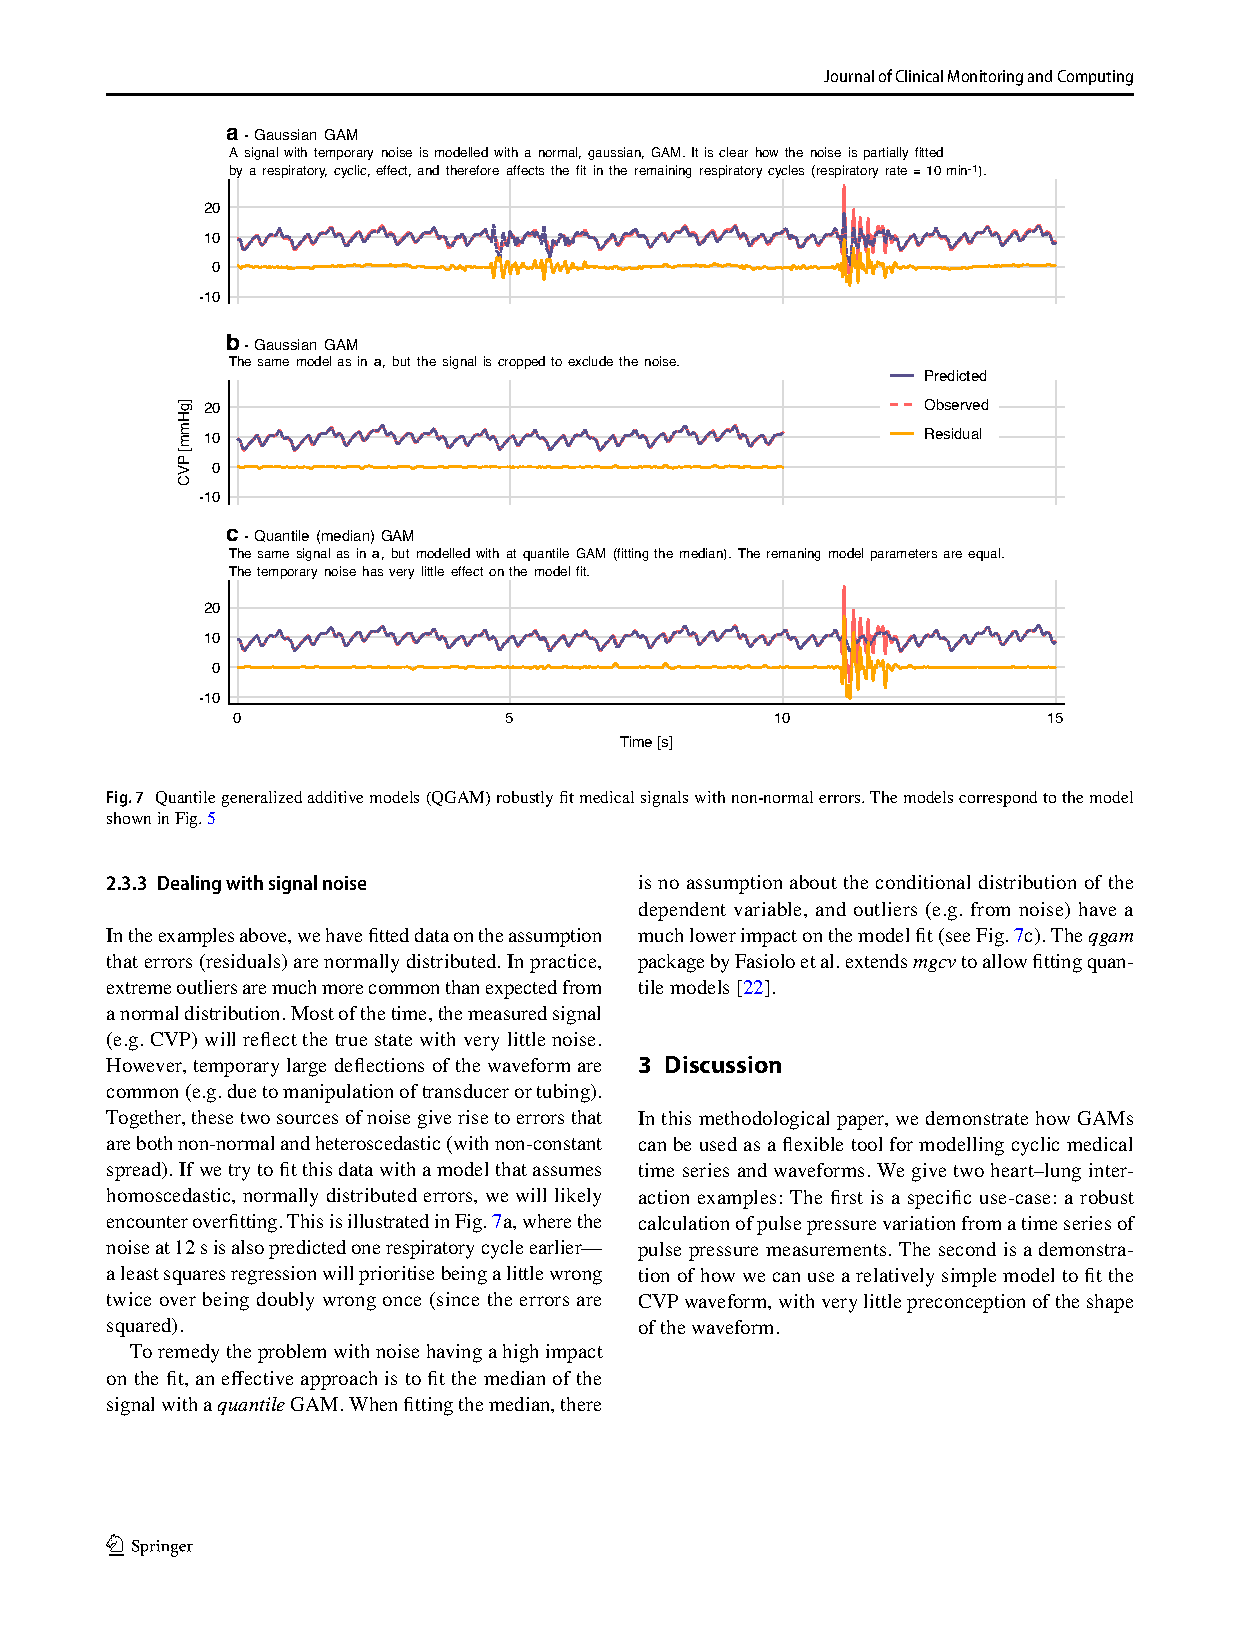
\includegraphics[width=1.2\linewidth]{papers/paper2//page-10.pdf}} \end{center} \newpage \begin{center} \makebox[\linewidth][c]{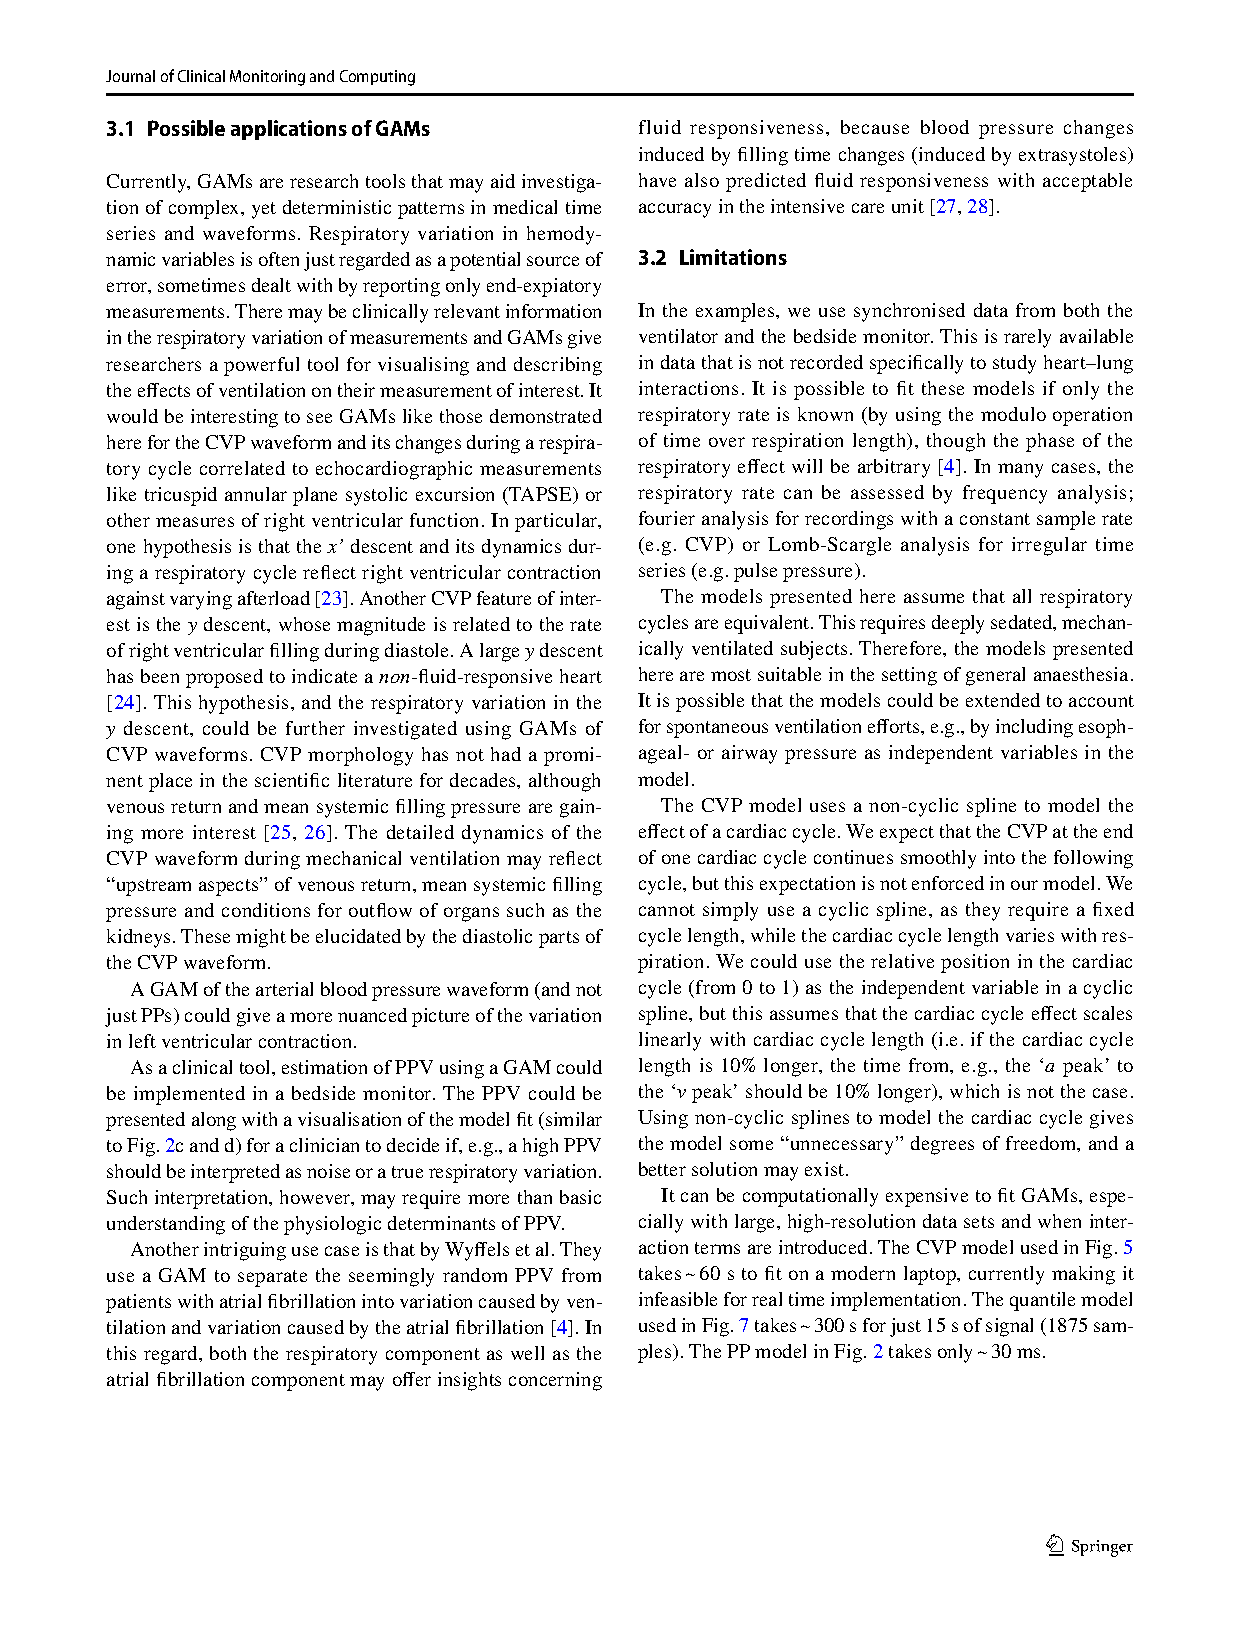
\includegraphics[width=1.2\linewidth]{papers/paper2//page-11.pdf}} \end{center} \newpage \begin{center} \makebox[\linewidth][c]{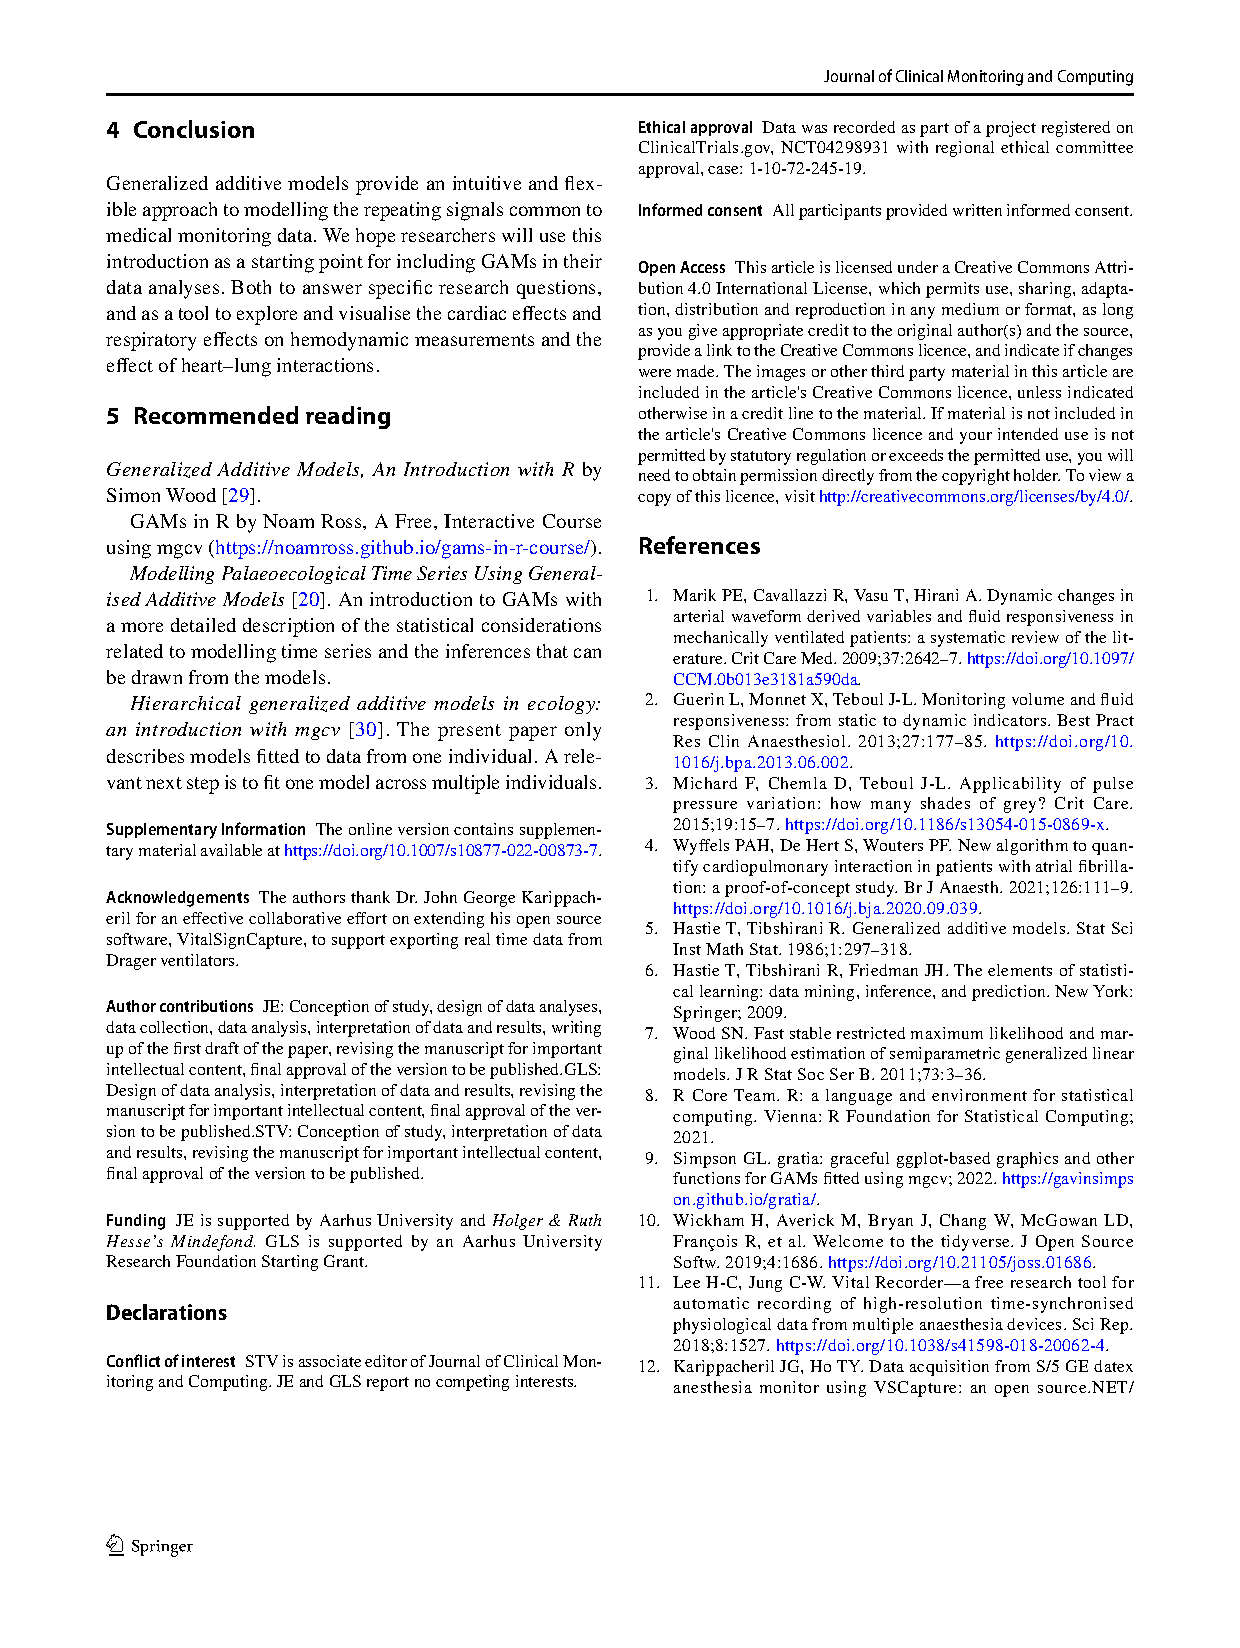
\includegraphics[width=1.2\linewidth]{papers/paper2//page-12.pdf}} \end{center} \newpage \begin{center} \makebox[\linewidth][c]{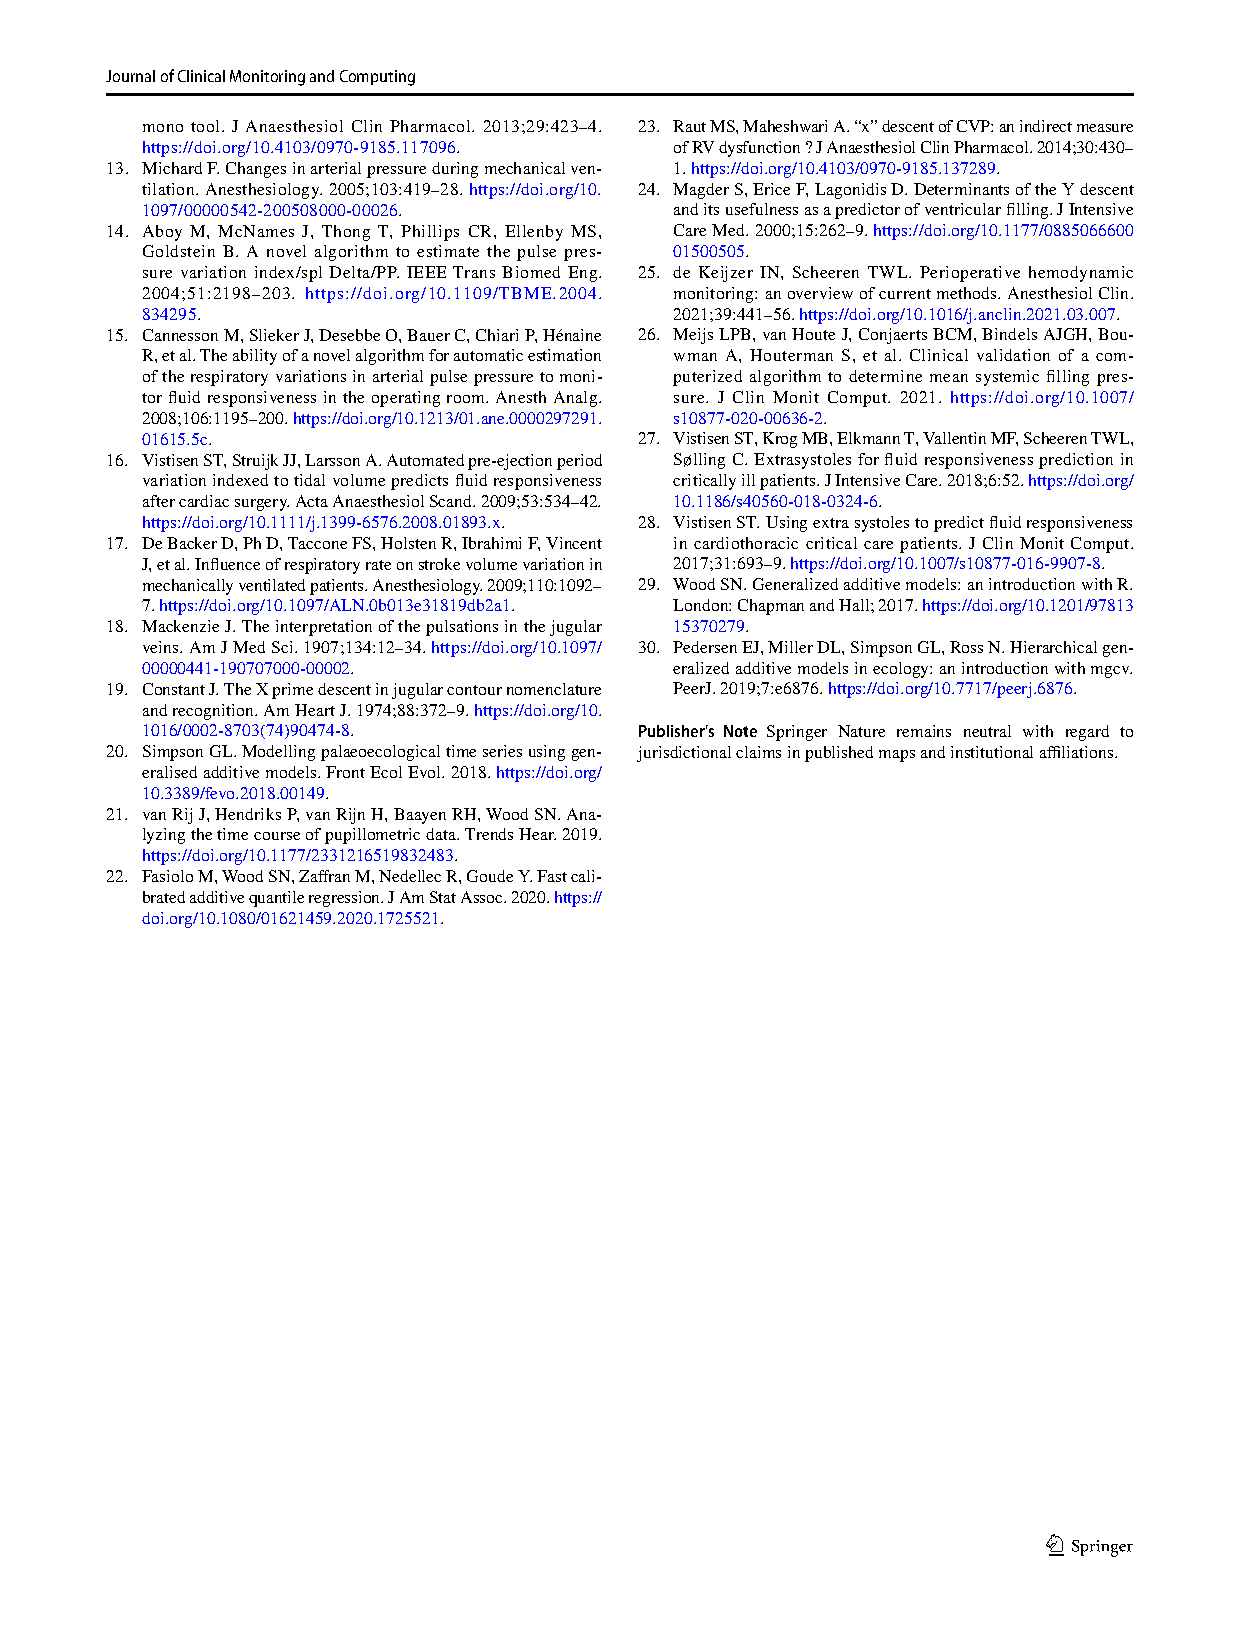
\includegraphics[width=1.2\linewidth]{papers/paper2//page-13.pdf}} \end{center} \newpage \begin{center} \makebox[\linewidth][c]{\includegraphics[width=1.2\linewidth]{papers/paper2//page-2.pdf}} \end{center} \newpage \begin{center} \makebox[\linewidth][c]{\includegraphics[width=1.2\linewidth]{papers/paper2//page-3.pdf}} \end{center} \newpage \begin{center} \makebox[\linewidth][c]{\includegraphics[width=1.2\linewidth]{papers/paper2//page-4.pdf}} \end{center} \newpage \begin{center} \makebox[\linewidth][c]{\includegraphics[width=1.2\linewidth]{papers/paper2//page-5.pdf}} \end{center} \newpage \begin{center} \makebox[\linewidth][c]{\includegraphics[width=1.2\linewidth]{papers/paper2//page-6.pdf}} \end{center} \newpage \begin{center} \makebox[\linewidth][c]{\includegraphics[width=1.2\linewidth]{papers/paper2//page-7.pdf}} \end{center} \newpage \begin{center} \makebox[\linewidth][c]{\includegraphics[width=1.2\linewidth]{papers/paper2//page-8.pdf}} \end{center} \newpage \begin{center} \makebox[\linewidth][c]{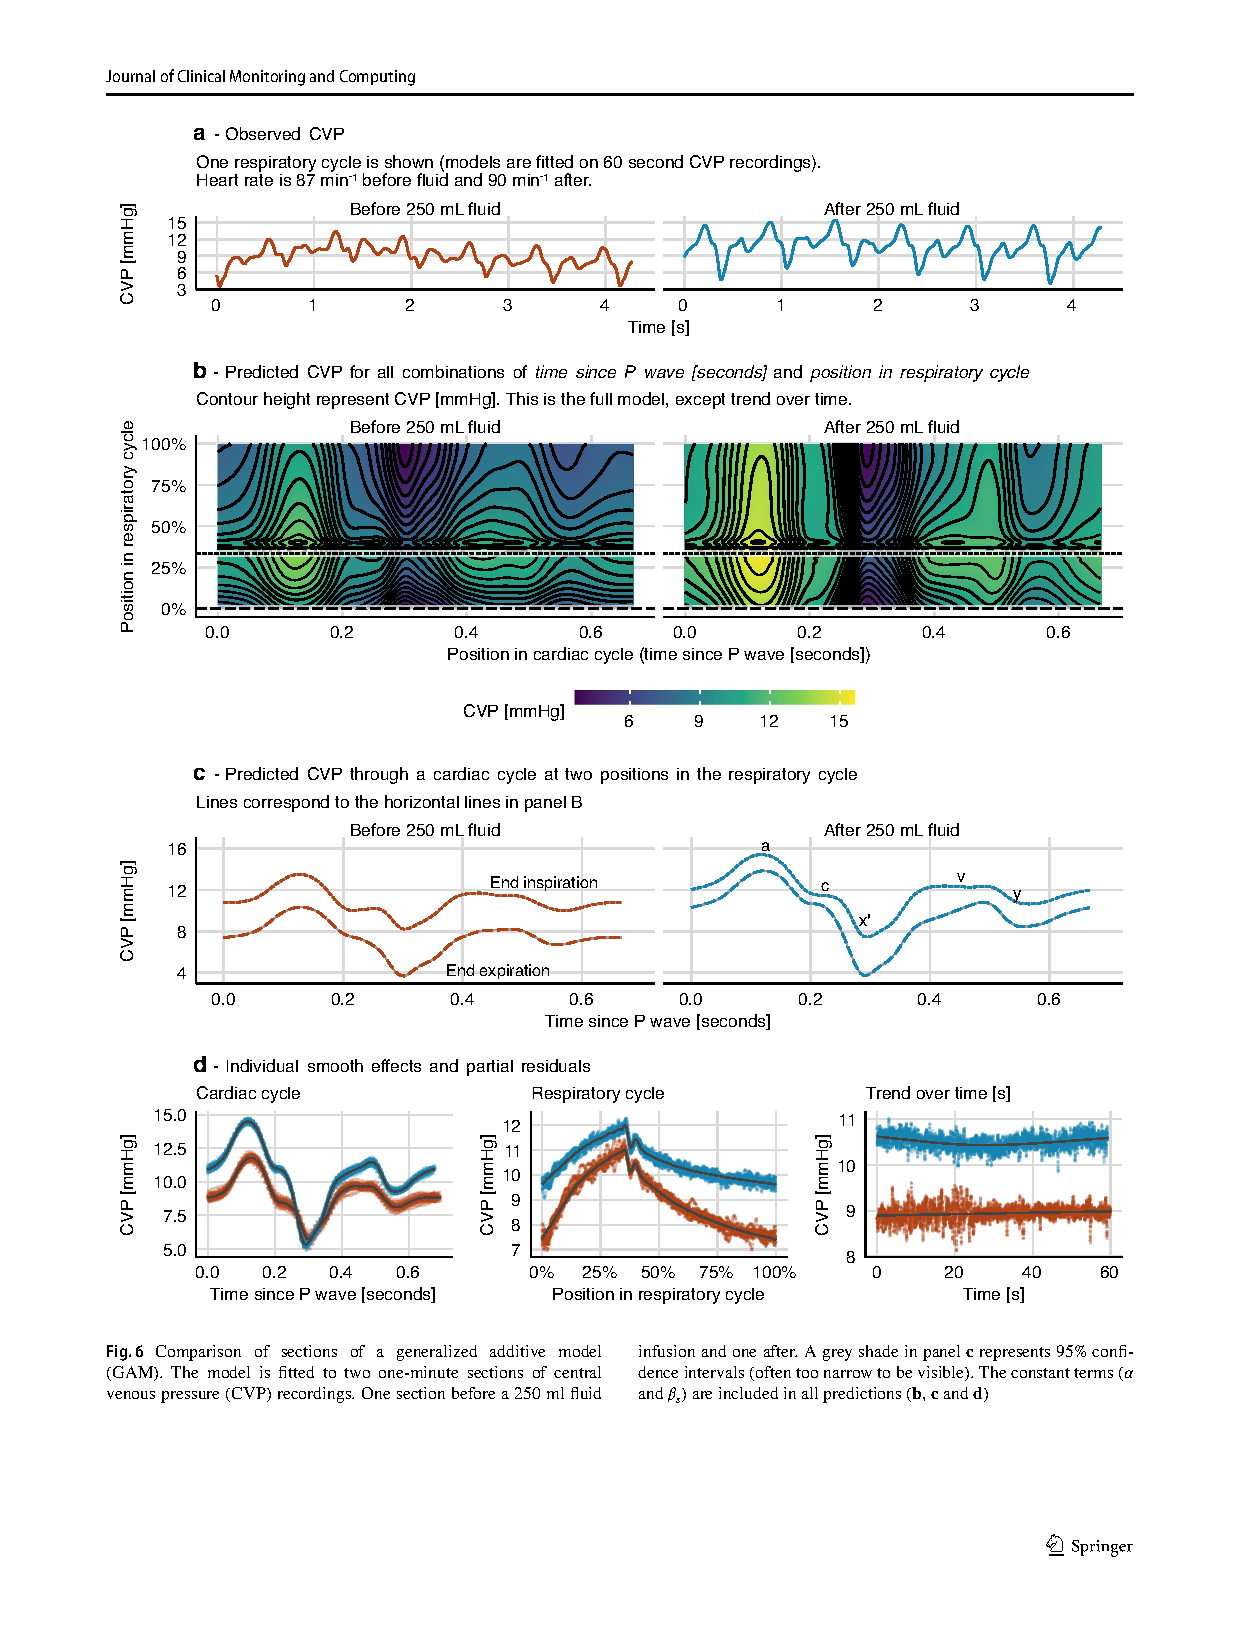
\includegraphics[width=1.2\linewidth]{papers/paper2//page-9.pdf}} \end{center}

\hypertarget{paper-3}{%
\chapter{Paper 3}\label{paper-3}}

\hypertarget{references}{%
\chapter*{References}\label{references}}
\addcontentsline{toc}{chapter}{References}

\hypertarget{refs}{}
\begin{CSLReferences}{0}{0}
\leavevmode\vadjust pre{\hypertarget{ref-bhaveVolumeDepletionDehydration2011}{}}%
\CSLLeftMargin{{[}1{]} }
\CSLRightInline{Gautam Bhave and Eric G. Neilson. 2011. Volume {Depletion Versus Dehydration}: {How Understanding} the {Difference Can Guide Therapy}. \emph{American Journal of Kidney Diseases} 58, 2 (August 2011), 302--309. DOI:https://doi.org/\href{https://doi.org/10.1053/j.ajkd.2011.02.395}{10.1053/j.ajkd.2011.02.395}}

\leavevmode\vadjust pre{\hypertarget{ref-coeCrystalloidPreloadingUseful1990}{}}%
\CSLLeftMargin{{[}2{]} }
\CSLRightInline{A.j. Coe and B. Revanäs. 1990. Is crystalloid preloading useful in spinal anaesthesia in the elderly? \emph{Anaesthesia} 45, 3 (1990), 241--243. DOI:https://doi.org/\href{https://doi.org/10.1111/j.1365-2044.1990.tb14696.x}{10.1111/j.1365-2044.1990.tb14696.x}}

\leavevmode\vadjust pre{\hypertarget{ref-cosnettOriginsIntravenousFluid1989}{}}%
\CSLLeftMargin{{[}3{]} }
\CSLRightInline{J. E. Cosnett. 1989. The origins of intravenous fluid therapy. \emph{Lancet (London, England)} 1, 8641 (April 1989), 768--771. DOI:https://doi.org/\href{https://doi.org/10.1016/s0140-6736(89)92583-x}{10.1016/s0140-6736(89)92583-x}}

\leavevmode\vadjust pre{\hypertarget{ref-foexHowCholeraEpidemic2003}{}}%
\CSLLeftMargin{{[}4{]} }
\CSLRightInline{B. A. Foëx. 2003. How the cholera epidemic of 1831 resulted in a new technique for fluid resuscitation. \emph{Emergency Medicine Journal} 20, 4 (July 2003), 316--318. DOI:https://doi.org/\href{https://doi.org/10.1136/emj.20.4.316}{10.1136/emj.20.4.316}}

\leavevmode\vadjust pre{\hypertarget{ref-jacobThirdSpaceFact2009}{}}%
\CSLLeftMargin{{[}5{]} }
\CSLRightInline{Matthias Jacob, Daniel Chappell, and Markus Rehm. 2009. The 'third space'--fact or fiction? \emph{Best Practice \& Research. Clinical Anaesthesiology} 23, 2 (June 2009), 145--157. DOI:https://doi.org/\href{https://doi.org/10.1016/j.bpa.2009.05.001}{10.1016/j.bpa.2009.05.001}}

\leavevmode\vadjust pre{\hypertarget{ref-kadetHouseCallsHangovers2015}{}}%
\CSLLeftMargin{{[}6{]} }
\CSLRightInline{Anne Kadet. 2015. House {Calls} for {Hangovers}. \emph{Wall Street Journal} (August 2015).}

\leavevmode\vadjust pre{\hypertarget{ref-lattaMALIGNANTCHOLERADOCUMENTS1832}{}}%
\CSLLeftMargin{{[}7{]} }
\CSLRightInline{Thomas Latta. 1832. {MALIGNANT CHOLERA}.: {DOCUMENTS COMMUNICATED BY THE CENTRAL BOARD OF HEALTH}, {LONDON}, {RELATIVE TO THE TREATMENT OF CHOLERA BY THE COPIOUS INJECTION OF AQUEOUS AND SALINE FLUIDS INTO THE VEINS}. \emph{The Lancet} 18, 457 (June 1832), 274--280. DOI:https://doi.org/\href{https://doi.org/10.1016/S0140-6736(02)80289-6}{10.1016/S0140-6736(02)80289-6}}

\leavevmode\vadjust pre{\hypertarget{ref-lewinsInjectionSalineSolutions1832}{}}%
\CSLLeftMargin{{[}8{]} }
\CSLRightInline{R Lewins. 1832. Injection of {Saline Solutions} into the {Veins}. \emph{BOSTON MEDICAL AND SURGICAL JOURNAL} VI, 24 (1832), 373--374.}

\leavevmode\vadjust pre{\hypertarget{ref-millerPerioperativeFluidTherapy2019}{}}%
\CSLLeftMargin{{[}9{]} }
\CSLRightInline{Timothy E. Miller and Paul S. Myles. 2019. Perioperative {Fluid Therapy} for {Major Surgery}. \emph{Anesthesiology} 130, 5 (May 2019), 825--832. DOI:https://doi.org/\href{https://doi.org/10.1097/ALN.0000000000002603}{10.1097/ALN.0000000000002603}}

\leavevmode\vadjust pre{\hypertarget{ref-monnetMyPatientHas2018}{}}%
\CSLLeftMargin{{[}10{]} }
\CSLRightInline{Xavier Monnet and Jean-Louis Teboul. 2018. My patient has received fluid. {How} to assess its efficacy and side effects? \emph{Annals of Intensive Care} 8, 1 (December 2018), 54. DOI:https://doi.org/\href{https://doi.org/10.1186/s13613-018-0400-z}{10.1186/s13613-018-0400-z}}

\leavevmode\vadjust pre{\hypertarget{ref-petroianuSalineInfusionClonus2021}{}}%
\CSLLeftMargin{{[}11{]} }
\CSLRightInline{Georg A Petroianu. 2021. On saline infusion, clonus, molecules and forgotten scientists: {Who} was {Dr Julius Sander} (1840\textendash 1909)? \emph{Journal of Medical Biography} (December 2021), 09677720211065357. DOI:https://doi.org/\href{https://doi.org/10.1177/09677720211065357}{10.1177/09677720211065357}}

\leavevmode\vadjust pre{\hypertarget{ref-smithPerioperativeFastingAdults2011}{}}%
\CSLLeftMargin{{[}12{]} }
\CSLRightInline{Ian Smith, Peter Kranke, Isabelle Murat, Andrew Smith, Geraldine O'Sullivan, Eldar Søreide, Claudia Spies, and Bas in't Veld. 2011. Perioperative fasting in adults and children: Guidelines from the {European Society} of {Anaesthesiology}. \emph{European Journal of Anaesthesiology \textbar{} EJA} 28, 8 (August 2011), 556--569. DOI:https://doi.org/\href{https://doi.org/10.1097/EJA.0b013e3283495ba1}{10.1097/EJA.0b013e3283495ba1}}

\end{CSLReferences}

%%%%% REFERENCES


\end{document}
